\documentclass[a4j,10.5pt,titlepage]{jarticle}
\usepackage[utf8]{inputenc}

\usepackage[dvipdfmx]{graphicx}
\usepackage{wrapfig}
\usepackage{amsmath}
\usepackage{tocloft}
\usepackage{geometry}

% ページの余白を1.25インチにする
\geometry{
	left=1.25truein,
	right=1.25truein,
	top=1.25truein,
	bottom=1.25truein,
}

% 目次の表題を、largeサイズ, 太字, 中央寄せに変更
\renewcommand{\cfttoctitlefont}{\hfill\large\bfseries}
\renewcommand{\cftaftertoctitle}{\hfill\null}
% 表題の上下の調整幅をなくす
\renewcommand{\cftbeforetoctitleskip}{0pt}
\renewcommand{\cftaftertoctitleskip}{0pt}

% 表目次の場合も同様
\renewcommand{\cftlottitlefont}{\hfill\large\bfseries}
\renewcommand{\cftafterlottitle}{\hfill\null}
\setlength{\cftbeforelottitleskip}{0pt}
\setlength{\cftafterlottitleskip}{0pt}
% 表番号の前に「Table」をつける
\renewcommand{\cfttabpresnum}{Table }
% 表番号の後に「:」をつける
\renewcommand{\cfttabaftersnum}{:}
% 表見出しのインデント幅
\renewcommand{\cfttabnumwidth}{6em}

% 図目次の場合も同様
\renewcommand{\cftloftitlefont}{\hfill\large\bfseries}
\renewcommand{\cftafterloftitle}{\hfill\null}
\setlength{\cftbeforeloftitleskip}{0pt}
\setlength{\cftafterloftitleskip}{0pt}
\renewcommand{\cftfigpresnum}{Figure }
\renewcommand{\cftfigaftersnum}{:}
\renewcommand{\cftfignumwidth}{6em}

%ページの上下に出力される図と図の間のスペース
\setlength\floatsep{5.0pt} %dblfloatsep

%ページの上下に出力される図と本文の間のスペース
\setlength\textfloatsep{5.0pt} %dbltextfloatsep

%ページの途中に出力される図と本文の間のスペース
\setlength\intextsep{5.0pt}

%図の参照
\newcommand{\Fig}[1]{Fig.\ref{fig:#1}}
%表の参照
\newcommand{\Tb}[1]{Tab.\ref{tab:#1}}
%式の参照
\newcommand{\Eq}[1]{Eq.(\ref{eq:#1})}

\renewcommand{\figurename}{Figure}
\renewcommand{\tablename}{Table}

\makeatletter
 \renewcommand{\theequation}{%
   \thesection.\arabic{equation}}
  \@addtoreset{equation}{section}
  
  \renewcommand{\thefigure}{
  \thesection.\arabic{figure}}
  \@addtoreset{figure}{section}
  
  \renewcommand{\thetable}{
    \thesection.\arabic{table}}
  \@addtoreset{table}{section}
\makeatother

\title{卒業論文}
\author{Ryohsuke Nishimoto}
\date{\today}

\begin{document}
\maketitle
\pagenumbering{roman}
\setcounter{tocdepth}{3}
\tableofcontents

\clearpage
\pagenumbering{arabic}

%%% ---- 序論 ---- %%%
\section{序論}
	%\input{intro/intro}
	
%%% ---- 理論 ---- %%%
\section{理論}
	\subsection{イオントラップ}
	\subsection{パウルトラップ}
	\subsection{プレーナーイオントラップ}
		\subsubsection{電極の仕様}
		\subsubsection{Single-well}
		\subsubsection{Double-well}
	\subsection{レーザー冷却}
	\subsection{イオンの運動}
		\subsubsection{余剰マイクロ運動}
	\subsection{画像処理によるイオン捕獲位置と電場の算出}
		\subsubsection{グレースケール化,二値化}
		\subsubsection{イオンの検出および,捕獲位置と電場の算出方法}

%%% ---- 実験のセットアップ ---- %%%
\chapter{実験装置}
\section{プレーナートラップ}
本実験で使用する電極の写真を\Fig{Using_PlannerTrap}に示す.
\begin{figure}[h]
	\begin{center}
		\includegraphics[width = 0.6\linewidth]{./experimental_setup/figure/Using_PlannerTrap.png}
		\caption{本実験で使用するプレーナートラップ}
		\label{fig:Using_PlannerTrap}
	\end{center}
\end{figure}

\section{光学系}
\Fig{optical_system}にイオン捕獲のためのレーザーの光学系を示す.
\begin{figure}[h]
	\centering
		\includegraphics[width = 0.7\linewidth]{./experimental_setup/figure/Optical_System.png}
		\caption{プレーナートラップに照射するレーザーの光学系}
		\label{fig:optical_system}
\end{figure}

\section{レーザー}
\begin{table}[h]
	\centering
		\caption{$^{40}{\rm Ca}^+$を捕獲するときに使用するレーザーの波長}
		\label{tb:use_laser}
			\begin{tabular}{c|c} \hline \hline
				基準周波数 & 632 nm \\ 
				$^{40}{\rm Ca}$のイオン化 & 423 nm, 375 nm \\
				$^{40}{\rm Ca}^+$の冷却 & 397 nm \\
				$^{40}{\rm Ca}^+$のリポンプ & 866 nm \\ \hline 
			\end{tabular}
\end{table}
イオントラップに使用するレーザーのビーム径とその強度をスリット走査型光ビームプロファイラ(THORLABS,BP209-VIS/M)とデジタルパワー\&エネルギーメータ(THORLABS,PM100D)およびフォトダイオードパワーセンサー(THORLABS,S120C)を用いて計測を行った.
まず,各レーザーの強度を\Tb{AllLaserPower}に示す.

\begin{table}[h]
	\begin{center}
		\caption{各レーザーのパワー一覧表}
		\label{tab:AllLaserPower}
		\begin{tabular}{c|c} \hline \hline
			波長 (nm) & 強度 ($\mu$W) \\ \hline
			375 &4.1 \\ \hline
			397 &17.4 \\ \hline
			423 &28.4 \\ \hline
			866 &700 \\ \hline
		\end{tabular}
	\end{center}
\end{table}

次に,ビーム径の計測結果を\Fig{AllLaserBeamProfile}に示す.

\begin{figure}[h]
	\begin{center}
	\begin{minipage}{0.48\linewidth}
		\includegraphics[width = 0.98\columnwidth]{./experimental_setup/figure/AllLaserXpos.jpg}
	\end{minipage}
	\begin{minipage}{0.48\linewidth}
		\begin{center}
		\includegraphics[width = 0.98\columnwidth]{./experimental_setup/figure/AllLaserYpos.jpg}
		\end{center}
	\end{minipage}
	\caption{4種類のレーザーのx,y方向についてのビームプロファイル結果}
	\label{fig:AllLaserBeamProfile}
	\end{center}
\end{figure}

そして,得られたビームプロファイルにガウシアンによるフィッティングを行った様子を\Fig{GaussianFitting}に示し,その結果を\Tb{GaussianFitting}にまとめている.\\

\begin{table}[h]
	\begin{center}
		\caption{ビームプロファイラで得られた各ビームのプロファイルにガウシアンフィッティングをかけて得られたパラメータ}
		\label{tab:GaussianFitting}
		\begin{tabular}{c|cc|cc} \hline \hline
			波長 (nm)&位置(x) ($\mu$m)&ビーム径(x) ($\mu$m) &位置(y) ($\mu$m)& ビーム径(y) ($\mu$m)\\ \hline
			375&-2600.82$\pm$0.035&6.96$\pm$0.049&-1051.14$\pm$0.028&9.37$\pm$0.04 \\
			397&-2606.08$\pm$0.026&24.21$\pm$0.037&-1056.17$\pm$0.016&18.45$\pm$0.023 \\
			423&-2611.55$\pm$0.05&30.20$\pm$0.072&1042.25$\pm$0.03&39.85$\pm$0.054 \\
			866&-2606.08$\pm$0.138&77.20$\pm$0.196&-1054.24$\pm$0.06&54.72$\pm$0.085 \\\hline
		\end{tabular}
	\end{center}
\end{table}

\clearpage

\begin{figure}[h]
	\begin{center}
	%%%12
	\begin{minipage}{0.48\linewidth}
	\begin{center}
			\includegraphics[width = 0.98\columnwidth]{./experimental_setup/figure/375GaussianFittingXpos.jpg}
	\end{center}
	\end{minipage}
	\begin{minipage}{0.48\linewidth}
	\begin{center}
			\includegraphics[width=0.98\columnwidth]{./experimental_setup/figure/375GaussianFittingYpos.jpg}
	\end{center}
	\end{minipage}
	%%%34
	\begin{minipage}{0.48\linewidth}
	\begin{center}
		\includegraphics[width = 0.98\columnwidth]{./experimental_setup/figure/397GaussianFittingXpos.jpg}
	\end{center}
	\end{minipage}
	\begin{minipage}{0.48\linewidth}
	\begin{center}
		\includegraphics[width=0.98\columnwidth]{./experimental_setup/figure/397GaussianFittingYpos.jpg}
	\end{center}
	\end{minipage}
	%%%56
	\begin{minipage}{0.48\linewidth}
	\begin{center}
		\includegraphics[width = 0.98\columnwidth]{./experimental_setup/figure/423GaussianFittingXpos.jpg}
	\end{center}
	\end{minipage}
	\begin{minipage}{0.48\linewidth}
	\begin{center}
		\includegraphics[width=0.98\columnwidth]{./experimental_setup/figure/423GaussianFittingYpos.jpg}
	\end{center}
	\end{minipage}
	%%%78
	\begin{minipage}{0.48\linewidth}
	\begin{center}
		\includegraphics[width = 0.98\columnwidth]{./experimental_setup/figure/866GaussianFittingXpos.jpg}
	\end{center}
	\end{minipage}
	\begin{minipage}{0.48\linewidth}
	\begin{center}
		\includegraphics[width = 0.98\columnwidth]{./experimental_setup/figure/866GaussianFittingYpos.jpg}
	\end{center}
	\end{minipage}
	\caption{各波長に対してx,y方向それぞれのビームプロファイルにガウシアンフィッティングをかけた結果}
	\label{fig:GaussianFitting}
	\end{center}
\end{figure}

\section{電気系}

%%% ---- 実験方法と実験結果 ---- %%%
\section{実験方法と結果}
	\subsection{一列配列イオン}
		\subsubsection{捕獲の手順}
		\subsubsection{イオン捕獲位置のdc電圧依存性}
		\subsubsection{永年周波数のdc電圧依存性}
		\subsubsection{シミュレーションとの比較}
	\subsection{二列配列イオン}
		\subsubsection{捕獲の手順}
		\subsubsection{比率Rとイオン列間距離の関係}
		\subsubsection{シミュレーションとの比較}
	
	\subsection{余剰マイクロ運動の補正}
		\subsubsection{補正の手順}
		\subsubsection{補正結果}
		
%%% ---- 考察 ---- %%%
\section{考察}
%%% ---- 結論と展望 ---- %%%
\section{結論と展望}
%%% ---- 謝辞 ---- %%%
\section*{謝辞}
%%% ---- 参考文献 ---- %%%
\begin{thebibliography}{99}
\end{thebibliography}


%\input{section2/text_section2}
%\input{section3/text_section3}
%\input{section4/text_section4}
%\input{section5/text_section5}
%\input{section7/text_section7}
%\input{BeamProfile/BeamProfile}
%\input{section6/text_section6}

\end{document}


%%%%%%%%%%%%%%%%%%%%%%%%%%%%%%%%%%%%%%%%%%%%%%%%%%%%%%%%%%%%%%%%%%%%%%%%%%%%%%%%%%%%%%%%

